\chapter{Problemdomäne Pressenplanung}
\label{chapter:problem}
In diesem Kapitel wird das Problem der Pressenplanung zunächst erläutert,
bevor die prädikatenlogische Modellierung des Problems in einem Modell erfolgt.
Abschließend wird das Modell um Optimierungsziele erweitert.

\section{Anforderungen}
\label{sec:anforderungen}
Im Pressenplanungsproblem sind drei Entitäten und deren Eigenschaften von elementarer Bedeutung: Pressen, Balken und Bauteile.
Diese haben jeweils die Eigenschaften Höhe, Breite und Länge.
Zusätzlich gibt es Holzlamellen, welche durch Zersägen eines sogenannten \textit{Endlosbretts} entstehen.
Dieses kann von einer Maschine \textit{scheinbar} endlos ausgegeben werden.
Höhe und Breite der Lamelle sind fest.
Lamellen werden vertikal zu Bauteilen verleimt, sodass Bauteile immer die Form eines Quaders haben.
Diese Verleimung ist der eigentliche Grund für die Notwendigkeit des Pressens.
Folgend eine Abbildung verleimter Lamellen:

\begin{figure}[h]
    \centering
    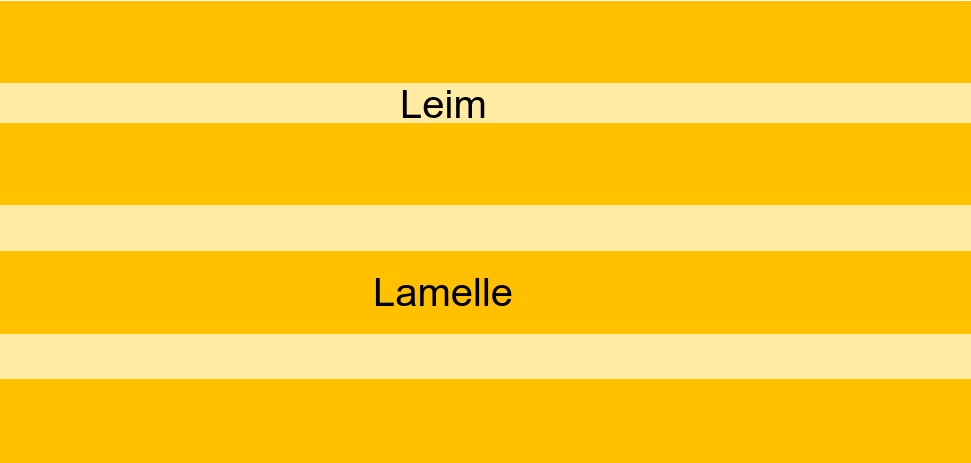
\includegraphics[width=0.70\textwidth, center]{Images/LammelleLeim}\\
    \caption{Vertikale Verleimung von Lamellen}
    \label{figure:lamelleleim}
\end{figure}

Bauteile wiederum formen Balken - ebenfalls Quader.
Bauteile erhält man durch vertikales Zersägen eines Balkens.
Folgend eine Abbildung eines Balkens aus drei Bauteilen mit Rest:

\begin{figure}[h]
    \centering
    
\includegraphics[width=1.00\textwidth, center]{Images/BalkenBauteileRest}\\
    \caption{Balken aus drei Bauteilen mit Rest, Sägelinien schwarz gepunktet}
    \label{figure:balkenbauteilerest}
\end{figure}

Balken werden vertikal in Pressen gestapelt und anschließend gepresst.
Eine mit Balken befüllte Presse, bei der festgelegt ist wie die Balken zu Bauteilen nach der Pressung zersägt werden müssen, nennt man auch Pressenplan.
In einem Pressenplan ist jedem Bauteil höchstens eine Position in einer Schicht (von unten gezählter Balken) einer Presse zugeordnet.
Folgend die Visualisierung eines Pressenplans für eine Presse:

\begin{figure}[h]
    \centering
    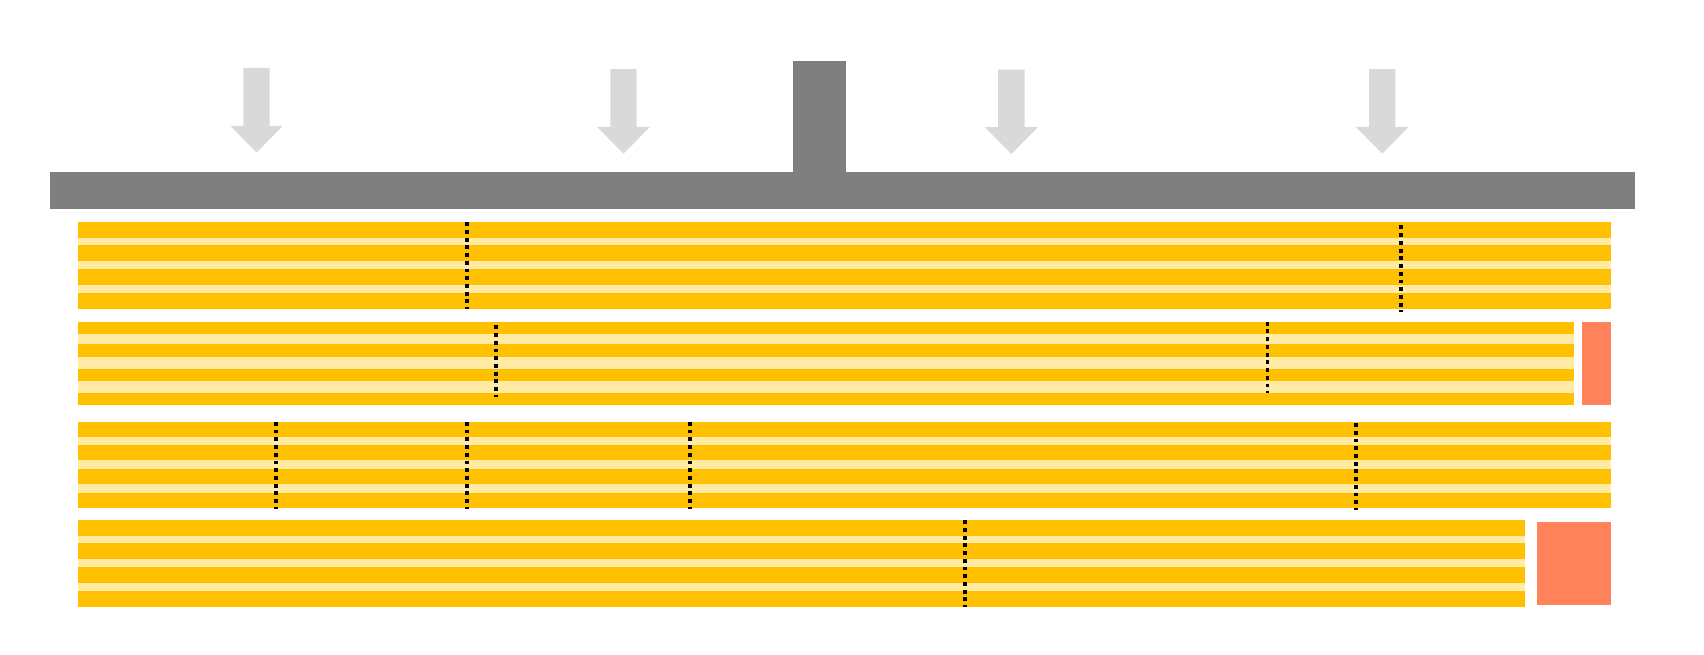
\includegraphics[width=1.00\textwidth, center]{Images/Pressenplan}\\
    \caption{Pressenplan für eine Presse mit vier Balken, 13 Bauteilen und zwei Reststücken}
    \label{figure:pressenplanproblem}
\end{figure}

Da Pressen im Allgemeinfall in einer Pressung nur Bauteile gleicher Breite pressen können, werden die Bauteile nach Breite vorsortiert.
Damit reduziert man die Dimension des Problems vom 3-Dimensionalen auf das 2-Dimensionale, da nur noch Länge und Höhe aller Entitäten berücksichtigt werden muss.

Die Eingabe für das Pressenplanungsproblem ist eine Liste von Bauteilen mit Länge und Höhe sowie deren Anzahl.
Diese Eingabe wird auch Auftrag genannt.
Folgend ein beispielhafter Auftrag:

\begin{table}[H]
    \centering
    \begin{tabular}{|c|c|c|}
        \hline
        \textbf{Länge in mm} & \textbf{Höhe in mm} & \textbf{Anzahl} \\
        \hline
        7000 & 400 & 1 \\
        13000 & 400 & 2 \\
        3000 & 400 & 3 \\
        6000 & 400 & 1 \\
        9000 & 400 & 1 \\
        7500 & 400 & 1 \\
        5000 & 400 & 1 \\
        5500 & 400 & 1 \\
        3500 & 400 & 1 \\
        \hline
    \end{tabular}
    \caption{Beispielauftrag, jede Zeile entpricht einer Bauteilspezifikation}
    \label{tab:auftrageingabe}
\end{table}

Die Lösung des Pressenplanungsproblems (Ausgabe) ist ein Pressenplan.
Für den Auftrag in Tabelle \ref{tab:auftrageingabe} könnte beispielsweise folgende Ausgabe den Pressenplan beschreiben:

\begin{table}[H]
    \centering
    \begin{tabular}{|c|c|c|c|c|}
        \hline
        \textbf{Presse} & \textbf{Schicht} & \textbf{Position} & \textbf{Länge in mm} & \textbf{Höhe in mm} \\
        \hline
        1 & 1 & 1 & 14000 & 400 \\
        1 & 1 & 2 & 7500 & 400 \\
        1 & 2 & 1 & 3000 & 400 \\
        1 & 2 & 2 & 6500 & 400 \\
        1 & 2 & 3 & 3000 & 400 \\
        \ldots & \ldots & \ldots & \ldots & \ldots \\
        \hline
    \end{tabular}
    \caption{Beispielausgabe des Pressenplans zu Auftrag in Tabelle \ref{tab:auftrageingabe}, Visualisierung in Abbildung \ref{figure:pressenplanproblem}}
    \label{tab:auftragausgabe}
\end{table}

An einen Pressenplan bestehen folgende Anforderungen:
\begin{itemize}
    \item Pressen haben eine Minimal- und Maximalhöhe. Die Summe der Höhe aller Balken einer Presse muss in diesem Intervall liegen.
    \item Pressen haben eine Minimal- und Maximallänge. Die Länge aller Balken einer Presse muss in diesem Intervall liegen.
    \item Alle Balken einer Presse haben die gleiche Länge. Dazu kann der Balken so aus Bauteilen zusammengesetzt sein, dass ein Rest übrig bleibt.
    \item Alle Bauteile, die einen Balken formen, haben die gleiche Höhe.
    \item Jedes Bauteil eines Auftrages ist höchstens einem Balken zugeordnet.
    \item Jeder Balken ist genau einer Presse zugeordnet.
\end{itemize}

% Hier könnte noch ein Beispiel eingefügt werden

\section{Modellierung}
\label{sec:modellierung}
In diesem Abschnitt wird ein mögliches Modell zur Modellierung des Pressenplanungsproblems erläutert.
Alle Namen von Funktionen in jenem Modell werden englisch formuliert, um die Nähe zur später in Abschnitt \ref{sec:kodierungconstraints} gezeigten Implementierung zu wahren.
Pressen heißen also \textit{Press}, Balken (Schichten) werden \textit{Layer} genannt und Bauteile erhalten den Namen \textit{Component}.
Die Menge aller Pressen wird mit $P$, die Menge aller Schichten mit $L$ und die Menge aller Bauteile mit $C$ abgekürzt.
Weiter werden boolesche als auch arithmetische Operatoren vorausgesetzt und in den Signaturen der Modelle nicht genannt.

\[
    \begin{aligned}
        \text{Folgend die Signatur } \Sigma = \left( \Sigma_{F}^{P} \cup \Sigma_{F}^{L} \cup \Sigma_{F}^{C}, \Sigma_{R} \right) \text{ mit Variablen } \mathbb{X} = \mathbb{X}^{P} \cup \mathbb{X}^{L} \cup \mathbb{X}^{C} \text{ wobei } \\[5pt]
            \begin{array}{ll}
                \begin{aligned}
                    \Sigma_{F}^{P} = \left\{
                    \begin{aligned}
                        & (id, & P \rightarrow \mathbb{N}_0), \\
                        & (minLength, & P \rightarrow \mathbb{N}_0), \\
                        & (maxLength, & P \rightarrow \mathbb{N}_0), \\
                        & (length, & P \rightarrow \mathbb{N}_0), \\
                        & (minHeight, & P \rightarrow \mathbb{N}_0), \\
                        & (maxHeight, & P \rightarrow \mathbb{N}_0), \\
                        & (height, & P \rightarrow \mathbb{N}_0), \\
                        & (layers, & P \rightarrow L_P \subseteq L)\; \\
                    \end{aligned} \right\} \\[5pt]
                \end{aligned}
                &
                \begin{aligned}
                    \mathbb{X}^{P} &= \bigcup_{p \in P} \left\{length(p), height(p) \right\} \\
                \end{aligned}
                \\
                \begin{aligned}
                    \Sigma_{F}^{L} = \left\{
                    \begin{aligned}
                        & (id, & L \rightarrow \mathbb{N}_0), \\
                        & (length, & L \rightarrow \mathbb{N}_0), \\
                        & (height, & L \rightarrow \mathbb{N}_0), \\
                        & (waste, & L \rightarrow \mathbb{N}_0), \\
                        & (isEmpty, & L \rightarrow \mathbb{B})\; \\
                    \end{aligned} \right\} \\[5pt]
                \end{aligned}
                &
                \begin{aligned}
                    \mathbb{X}^{L} &= \bigcup_{l \in L} \left\{length(l), height(l), waste(l), isEmpty(l)\right\} \\
                \end{aligned}
                \\
                \begin{aligned}
                    \Sigma_{F}^{C} &= \left\{
                    \begin{aligned}
                        & (length, & C \rightarrow \mathbb{N}_0), \\
                        & (height, & C \rightarrow \mathbb{N}_0)\; \\
                    \end{aligned} \right\} \\
                \end{aligned}
                &
                \begin{aligned}
                    \mathbb{X}^{C} &= \emptyset \\
                \end{aligned}
                \\[10pt]
                \begin{aligned}
                    \Sigma_{R} &= \left\{
                    \begin{aligned}
                        & (InLayer, C \times L \rightarrow \mathbb{B}) \\
                    \end{aligned} \right\} \\
                \end{aligned}
                &
                \begin{aligned}
                    \mathbb{X}^{InLayer} &= InLayer \\
                \end{aligned}
            \end{array}\\[5pt]
    \end{aligned}
\]
Damit lassen sich folgende Constraints formulieren:
\begin{align}
    & \forall p \in P: minHeight(p) \leq height(p) \leq maxHeight(p) \\[10pt]
    & \forall p \in P: minLength(p) \leq length(p) \leq maxLength(p) \\[10pt]
    & \forall p \in P,\; \forall l \in layers(P): \neg isEmpty(l) \rightarrow length(p) = length(l) \\[10pt]
    & \forall c \in C,\; \forall l \in L: InLayer(c,l) \rightarrow height(c) = height(l) \\[10pt]
    & \forall c \in C: atMost(1,\{ InLayer(c,l) \mid l \in L \}) \\[10pt]
    & \forall l \in L: isEmpty(l) \leftrightarrow \neg\bigvee_{c \in C} InLayer(c,l) \\[10pt]
    & \forall l \in L: isEmpty(l) \leftrightarrow (length(l) = 0 \land height(l) = 0) \\[10pt]
    & \forall p \in P: height(p) = \sum_{\substack{l \in layers(P)}} height(l)  \\[10pt]
    & \forall l \in L: length(l) = waste(l) + \sum_{\substack{c \in C}}
    \begin{cases}
        length(c) & \text{, } InLayer(c,l) \\
        0 & \text{, sonst}
    \end{cases}
\end{align}

\section{Optimierung}
Das obige Modell beschreibt beliebige Lösungen für das Problem der Pressenplanung.
Um Kosten- und Zeitaufwand beim Pressen zu reduzieren, sind Pressenpläne zusätzlich nach folgenden Kriterien lexikografisch zu optimieren (Vorgabe Germanedge):
\begin{enumerate}
    \item $ \min \left( \left\lvert \left\{ c \in C \mid \neg\bigvee\limits_{\substack{l \in L}} InLayer(c,l) \right\} \right\rvert \right) $
    \item $ \min (\lvert P \rvert) $
    \item $ \min \left(\sum\limits_{\substack{l \in L}} waste(l) \right) $
\end{enumerate}
